%!TEX root = ../reports.tex
%
% 磁場の性質
% レポート用紙
%

\stepcounter{section}
\section*{磁場の性質}

\begin{center}
\begin{tabular}{|c|c|c|c|}
\hline
\parbox[c][1.2cm][c]{0cm}{}学籍番号 & \hspace{3cm} & 名前 & \hspace{6cm} \\
\hline
\parbox[c][1.2cm][c]{0cm}{}実験日時 & \multicolumn{3}{|l|}{   年  月  日  曜日  時限}\\
\hline
\parbox[c][2.0cm][c]{0cm}{}共同実験者 & \multicolumn{3}{|l|}{}\\
\hline
\end{tabular}
\end{center}

\subsection*{実験の目的}

\vspace{6cm}

\subsection*{実験の記録}

%\subjikken{}
%\subsubsection*{鉄や鉄以外の物の磁石に対する反応}
%
%\newpage
%
%\subjikken{}
%\subsubsection*{電磁石のコイルの内側に鉄心を入れた時の変化}
%
%\vspace{5cm}


\subjikken{立体磁界観察槽で観察した磁場の様子(スケッチ)}
\begin{center}
\vspace{1cm}
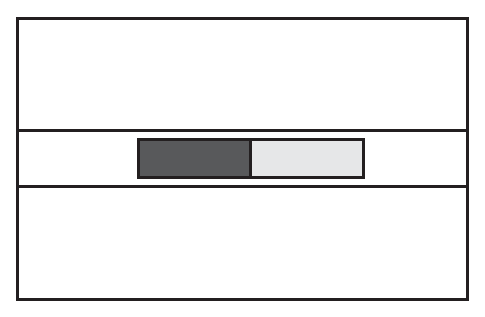
\includegraphics[scale=0.87]{06_Magnetism/magnet1.eps}
\hspace{1cm}
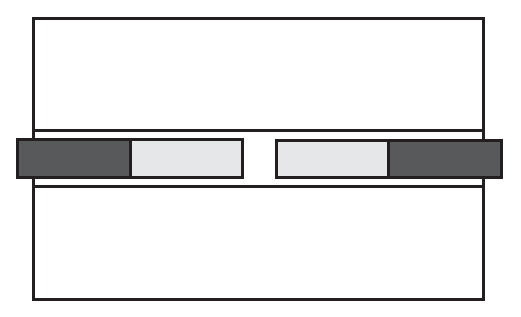
\includegraphics[scale=0.87]{06_Magnetism/magnet2.eps}
\end{center}

\newpage

%\subjikken{}
%\subsubsection*{地磁気の観察}
%
%\vspace{4cm}

\subjikken{磁界観察シートによる磁性体の様子(スケッチ)}
\vspace{7cm}

\subjikken{磁石の種類による磁力の違い}

\begin{center}
\begin{tabular}{|p{5cm}|p{3cm}|p{3cm}|}
\hline
磁石の種類 & 測定位置 [cm] &磁束密度 [mT]\\
\hline
&&\\
\hline
&&\\
\hline
&&\\
\hline
&&\\
\hline
&&\\
\hline
&&\\
\hline
\end{tabular}
\end{center}

\vspace{1cm}

\subjikken{磁場と磁化の測定}


\begin{center}
\begin{tabular}{|c|p{4.5cm}|}
\hline
電流 [A] & 鉄心上の磁束密度 [mT] \\
\hline
 &\\
\hline
 &\\
\hline
 &\\
\hline
&\\
\hline
&\\
\hline
&\\
\hline
&\\
\hline
&\\
\hline
&\\
\hline
&\\
\hline
&\\
\hline
\end{tabular}
\begin{tabular}{|c|p{4.5cm}|}
\hline
電流 [A] & 鉄心上の磁束密度 [mT] \\
\hline
&\\
\hline
&\\
\hline
&\\
\hline
&\\
\hline
&\\
\hline
&\\
\hline
&\\
\hline
&\\
\hline
&\\
\hline
&\\
\hline
&\\
\hline
\end{tabular}
\end{center}

\newpage

%\noindent
%4.0$\sim$5.0 [A]での鉄心上の磁束密度 [mT]から求めた電流$I$ [A]と外部磁束密度$B$ [mT]の関係
%\[
%B = a\times I, \qquad  a=\fbox{\hspace{2cm}} \text{ [mT/A]}
%\]




\subsubsection*{コイルの電流と鉄心上の磁束密度のグラフ}

\noindent
%鉄心上の磁束密度から外部磁束密度を引いたものを鉄心の磁化とし、
コイルに与えた電流(横軸)と鉄心上の磁束密度(縦軸)のグラフをプロットしなさい。

\bigskip

\hspace*{-\parindent}
\includegraphics[scale=0.83]{06_Magnetism/graph.eps}

\newpage

\subsection*{考察}

\begin{itemize}

\item 磁場の観察から磁力線にはどのような性質があるといえるでしょうか?

\vspace{6cm}
%\newpage

\item コイルに与えた電流と鉄心上の磁束密度の関係からどのようなことがわかるでしょうか?

\vspace{6cm}

\item 今回の実験で見たような磁石(磁場)の性質を用いたものとして、身の回りにどのようなものがあるでしょうか? 調べてみましょう。

\end{itemize}
